  %%%%%%%%%%%%%%%%%%%%%%%%%%%%%%%%%%%%%%% -*- coding: utf-8; mode: latex -*- %%
  %
%%%%%                       CHAPTER
 %%%
  %

\chapter{Results and discussion}
%\addcontentsline{lof}{chapter}{\thechapter\quad Nihil Molestiae}
%\addcontentsline{lot}{chapter}{\thechapter\quad Nihil Molestiae}
\label{ch:omnisvoluptas}

%\begin{quotation}
%  {\small\it Neque porro quisquam est qui dolorem ipsum quia dolor sit amet, consectetur, adipisci velit...}

%{\small\it -- Cerico}
%\end{quotation}


\section{Classification Experiments}

In this work, three types of experiments were conducted, each using two different architectures, as described in the previous chapter. Results are shown in tables \textbf{5.1} and \textbf{5.2} (for the baseline experiments), \textbf{5.3} and \textbf{5.4} (for the semi-independent experiments), and \textbf{5.5} and \textbf{5.6} (for the language-independent experiments). These tables show the five MLP parameter parameterizations with higher accuracy for each experiment. Tables \textbf{5.1}, \textbf{5.3} and \textbf{5.5} present the results for architecture 1, whereas tables \textbf{5.2}, \textbf{5.4} and \textbf{5.6} show the results for architecture 2.

\subsection{Baseline experiments}

Both architectures 1 and 2 of the \gls{mlp} yielded an accuracy of 90\% with the best parameterization (Tables \textbf{5.1} and \textbf{5.2}). \\
All the best models parameterizations (for both architectures 1 and 2) achieved higher scores using the GITA dataset. There are multiple reasons that can explain these results. In particular , the text read by subjects for the creation of the Gita dataset contains the complete set of Spanish sounds, which makes the data phonetically complete. Also, the audios from the MDVR\_KCL dataset were recorded using phone calls, which uses audio compression with data loss, resulting in a dataset with inferior quality. In addition, MDVR\_KCL has a significantly smaller recording time, which may limit the model learning. \\
The distribution between \gls{mlp} solvers (adam and lbfgs) on the top 5 model parameterizations for architecture 1 is similar, whereas 4 out of the 5 best model parameterizations on architecture 2 use the adam solver. Both architectures yielded better results when using valuer smaller values (0.0001 and 0.001) for the alpha parameter, comparing to the results obtained using larger values (0.1). Finally, architecture 1 does not show significant differences between models using 2000 and 5000 for the maximum number of iterations. In addition, this difference is observable on architecture 2, where the four model configurations which yielded better results by using the value of 5000 for this parameter regardless of the solver. The difference between architectures can be explained by the higher complexity of architecture 2 which require the optimization of a large number of parameters (52400 weights and 401 biases), compared with architecture 1, which has only 3844 weights and 63 bias. A larger number of parameters requires more iterations for the model's convergence. \\
Architecture 1 yielded precision values between 0.75 and 1, meaning that 75\% to 100\% of the patients labeled as \gls{pd} by the models were correctly classified. The precision of architecture 2 was slightly worse, between 67\% and 100\%. Recall values (which corresponds to the percentage of \gls{pd} patients were correctly classified) were similar for the two architectures. Architecture 1 led to recall values in the ranges [71-100]\% and [67-100]\%, respectively. Using the specificity metric (which corresponds to the percentage of \gls{hc} patients that were correctly classified) to compare the two architectures, architecture 2 outperformed architecture 1 by a small margin, producing a range of values between 80\% and 100\%, whereas architecture 1 produced a range of values between 75\% and 100\%. Finally, comparing both architectures using the F1-score metric, the performance of architecture 2 (up to 91\%) is usually higher than the one of architecture 2 (up to almost 86\%). \\
Overall, we can conclude that there are no significant differences between the two architectures.

\begin{table}
	\centering
	\begin{tabular}{lcccccccc}
		\bfseries dataset & \bfseries solver & \bfseries alpha & \bfseries max. iterations & \bfseries accuracy  & \bfseries precision & \bfseries recall & \bfseries specificity & \bfseries f1-score
		\csvreader[head to column names]{csvs/baseline_top.csv}{}
		{\\\hline\dataset & \solver & \alpha & \iterations & \accuracy  & \precision & \recall & \specificity & \fscore}
	\end{tabular}
	\caption{\label{tab:table-name}Baseline experiment results using architecture 1.}
\end{table}

\begin{table}
	\centering
	\begin{tabular}{lcccccccc}
		\bfseries dataset & \bfseries solver & \bfseries alpha & \bfseries max. iterations & \bfseries accuracy  & \bfseries precision & \bfseries recall & \bfseries specificity & \bfseries f1-score
		\csvreader[head to column names]{csvs/baseline_200_top.csv}{}
		{\\\hline\dataset & \solver & \alpha & \iterations & \accuracy  & \precision & \recall & \specificity & \fscore}
	\end{tabular}
	\caption{\label{tab:table-name}Baseline experiment result using architecture 2.}
\end{table}

\subsection{Semi-independent experiments}

When testing a semi-independent approach, architecture 1 yielded better results than architecture 2 (tables \textbf{table 5.3} and \textbf{table 5.4}). Although the two best model parameterization of both architectures produced an accuracy of 90\%, the following three model parameterization resulted in an accuracy of almost 86\%, whereas architecture 2 only reached an accuracy of 80\%. The same trend applies to precision.
\\
Architecture 1 outperformed architecture 2 on precision, producing results between 0.83 and 1, whereas architecture 2 yielded values between 0.6 and 1. While both architectures' highest value was the same, architecture 1 produced consistently better results, with a smaller range of values. Similar results were achieved when using recall. Architecture 1 produced values between 0.75 and 1, and 3 of the top 5 model parameterizations achieved 100\% recall. Additionally, architecture 2 values for recall ranged from 0.66 and 1. As F1-score combines the values from precision and recall (and architecture 1 outperformed architecture 2 on both these metrics), the F1-score metric leads to the same conclusions. Values of this metric for architecture 1 varied between 0.85 and 0.92, whereas architecture 2 values ranged from 0.75 to 0.88. Finally, architecture 2 produced better results when using specificity. This architecture's values varied between 0.71 and 1, with a much smaller variation between extremes when compared to the results produced by architecture 1, which varied from 0.5 to 1.
The results were similar to the ones achieved on the baseline experiences using architecture 2. Architecture 1 had a slightly better performance on the semi language-independent experiments, compared to the baselines.
This experiment confirms the conclusions of similar work that tested semi language-independent models \cite{parkinson_three_languages}, which suggests that these models can be retrained using a small dataset of a new language. These retrained models can be used on patients that speak the different language, without loss of performance. This characteristic can be particularly useful, as lack of training data is usually a limitation to train such models.

\begin{table}
	\centering
	\begin{tabular}{lcccccccc}
		\bfseries dataset & \bfseries solver & \bfseries alpha & \bfseries max. iterations & \bfseries accuracy  & \bfseries precision & \bfseries recall & \bfseries specificity & \bfseries f1-score
		\csvreader[head to column names]{csvs/semi_top.csv}{}
		{\\\hline\dataset & \solver & \alpha & \iterations & \accuracy  & \precision & \recall & \specificity & \fscore}
	\end{tabular}
	\caption{\label{tab:table-name}Semi-independent experiment result using architecture 1.}
\end{table}

\begin{table}
	\centering
	\begin{tabular}{lcccccccc}
		\bfseries dataset & \bfseries solver & \bfseries alpha & \bfseries max. iterations & \bfseries accuracy  & \bfseries precision & \bfseries recall & \bfseries specificity & \bfseries f1-score
		\csvreader[head to column names]{csvs/semi_200_top.csv}{}
		{\\\hline\dataset & \solver & \alpha & \iterations & \accuracy  & \precision & \recall & \specificity & \fscore}
	\end{tabular}
	\caption{\label{tab:table-name}Semi independent experiment result using architecture 2.}
\end{table}

\subsection{Language-independent experiments}

Language-independent models lead to substantially worse results compared to previous models (tables \textbf{table 5.5} and \textbf{table 5.6}). \\
When using a language-independent model, architecture 1 achieved a maximum accuracy of 67\%. Architecture 2 yielded very similar results, scoring a maximum of 66\% on this metric. \\
Combining the top five model parameterizations for both architectures, almost all (90\%) obtained their best scores when trained with the FraLusoPark and MDVR\_KCL, and tested with Gita. The same percentage of the combination of the top five models of each architecture used the \textit{lbfgs} solver, whereas only 1 of these 10 model parameterizations used the \textit{adam} solver. Similarly to the dependent and semi-independent experiments, the model's performance is consistently higher for smaller values of alpha. On both architectures, only 1 of the top five model parameterizations used $alpha = 1$. Finally, no significant differences were found when comparing model's performance based on the number of iterations. \\
Considering the precision metric, architecture 1 scored slightly higher values than architecture 2. It's values range between 0.59 and 0.64 whereas architecture 2 yielded values between 0.57 and 0.61, meaning that architecture 2 produced more false positives (patients from the \gls{hc} group incorrectly classified as \gls{pd}). Also, architecture 1 performed slightly worse when comparing the recall metric, only achieving values ranging from 0.76 to 0.84, whereas architecture 2 scored recall values between 0.77 and 0.88, thus correctly classifying a higher number of patients from the \gls{pd} group. Architecture 1 outperformed architecture 2, when compared using the specificity metric. Architecture 2 only achieved a maximum of 0.46, compared to architecture 1, which scored a maximum of 0.58 on this metric. Lastly, as F1-score combines precision and recall in the same metric, the results of both architectures on this metric were equivalent. \\
We can conclude that the models have a similar performance on the \gls{pd} detection task. Thus, Architecture 1 can be considered a better option for this task, as it is simpler, with only 3783 parameters to optimize, than architecture 2, which comprises a total of 52601 parameters. This difference makes architecture 1 much less resource-intensive, in both terms of time and computing power.

\begin{table}
	\centering
	\begin{tabular}{lcccccccc}
		\bfseries dataset & \bfseries solver & \bfseries alpha & \bfseries max. iterations & \bfseries accuracy  & \bfseries precision & \bfseries recall & \bfseries specificity & \bfseries f1-score
		\csvreader[head to column names]{csvs/independent_top.csv}{}
		{\\\hline\dataset & \solver & \alpha & \iterations & \accuracy  & \precision & \recall & \specificity & \fscore}
	\end{tabular}
	\caption{\label{tab:table-name}Independent experiment result using architecture 1.}
\end{table}

\begin{table}
	\centering
	\begin{tabular}{lcccccccc}
		\bfseries dataset & \bfseries solver & \bfseries alpha & \bfseries max. iterations & \bfseries accuracy  & \bfseries precision & \bfseries recall & \bfseries specificity & \bfseries f1-score
		\csvreader[head to column names]{csvs/independent_200_top.csv}{}
		{\\\hline\dataset & \solver & \alpha & \iterations & \accuracy  & \precision & \recall & \specificity & \fscore}
	\end{tabular}
	\caption{\label{tab:table-name}Independent experiment result using architecture 2.}
\end{table}

\subsection{Model optimization}

When comparing models' results per parameter, it is possible to find the best values for each parameter. \\
Smaller values for alpha (0.0001 and 0.001) consistently produced superior results when compared with 0.01. Considering language-dependent and semi language-dependent models, there is no clear difference between the use of the lbfgs and adam solvers. For both experiments, around half of the top five model parameterizations used each solver. In addition, for language-independent experiments, models using the lbfgs solver outperformed those using the adam solver. Between the top five model parameterizations of each architecture, only 1 was trained using adam (tables \textbf{5.5} and \textbf{5.6}). Lastly, comparing the results based on the number of maximum number of iterations ($\#interations$), there is no clear difference between models trained with $\#iterations = 2000$ and $\#iterations = 5000$ in any of the experiments performed. This shows that, in most cases, 2000 iterations should be sufficient to train the model, and convergence is reached without executing the maximum number of iterations.

\section{Language Independency}

Both architectures used during this work yielded an accuracy of 90\% on the semi language-independent experiments. One the one hand, these results are inferior to the ones achieved on a similar work (\cite{parkinson_three_languages}), where the authors were able to achieve a maximum accuracy of 96\% when training a model with a German dataset and 80\% of a Spanish dataset and testing with the remaining 20\%. On the other hand, this model was outperformed by architecture 1 when using the recall metric, producing recall values of 95\%, whereas architecture 1 produced a recall of 100\% for the top 3 model parameterizations. Contrary to this work, results produced by our model were inferior when using the specificity metric, where the authors were able to achieve a score of 97\%, compared to the 75\% produced by our model. Based on the recall metric, we can conclude that our solution has better ability to indicate when a subject belongs in the \gls{pd} group. This contrasts with the ability to classify subjects from the \gls{hc} group, where our model has an inferior performance. As previously described in section 5.1.3, architecture 1 produced an accuracy of 67\% on the language-independent experiments. This result is slightly inferior to the one achieved on a different article \cite{parkinson_three_languages}, where a language-independent model yielded an accuracy of 77\% when trained with a Czech dataset and tested with a German dataset. Comparing the models using the recall and specificity metrics, the results are identical to the ones achieved on the semi language-independent models' comparison in this work. Our model produced a recall of 76\% whereas the authors were only able to score 53\% on this metric. On the other hand, architecture 1 produced a score of 58\% on the specificity metric, significantly inferior to the 95\% achieved by the other work. \\
It is possible to conclude that the performance of both architectures used in this work were not able to produce results at the state-of-the-art on the language independency topic. Regarding the recall metric, both architectures outperformed the state-of-the-art, which demonstrates better capacity in detecting \gls{pd}.

\section{Explainability}

LIME was used to generate explanations for each test subject. These are local explanations, as they are able to explain the classification of each test subject. Results obtained following this process are described in section 5.3.1. By analyzing the complete set of explanations produced in this work, the global contribution (weight) of each feature was evaluated for the classification. Results for the global analysis are described in section 5.3.2.

\subsection{Local Explanations}

\begin{figure*}[t]
	\begin{center}
		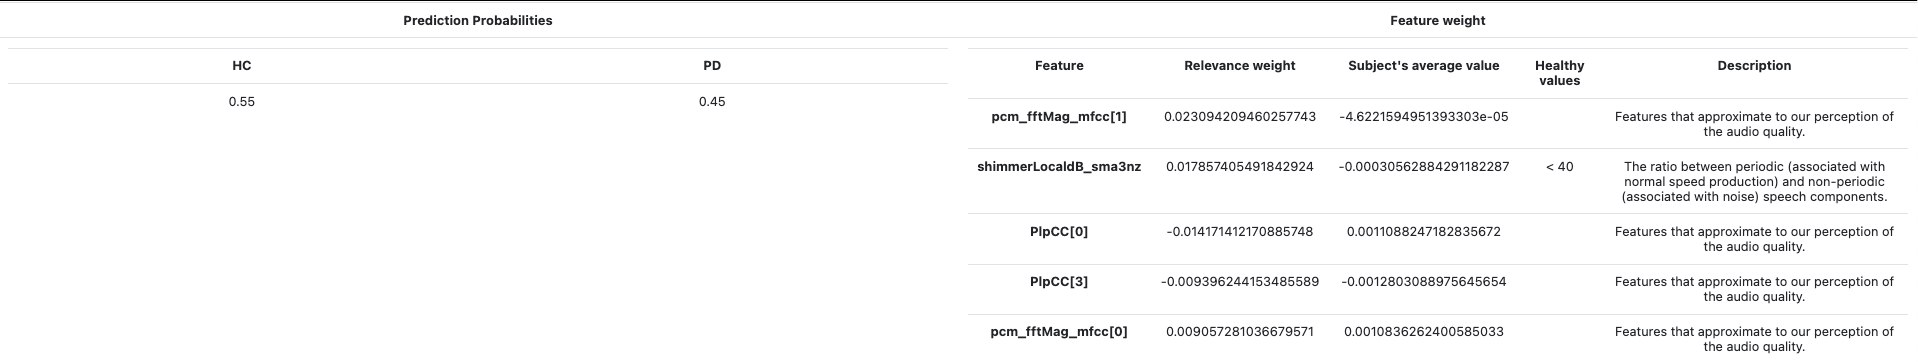
\includegraphics[clip=true, width=\textwidth]{figs/example_explanation.png}
	\end{center}
	\caption{Example of an explanation generated by LIME.}
	\label{explanation}
\end{figure*}

To generate an explanation, the top 5 features with the highest contribution to the diagnostic are selected. Figure \ref{explanation} illustrates an explanation, containing the percentage attributed to each class (\gls{pd} and \gls{hc}), the features with the highest contribution to the diagnostic, their corresponding weights, the subject's average value on that feature, the range of normal values for a healthy subject (extracted from the bibliography), and a short description of the feature. This information provides a clearer insight of the model's
classification to the medical professional. The percentage attributed to each class allows to evaluate the degree of confidence of the model in the decision, whereas the average features values can be compared to the normal range of values to check for abnormal parameters. Finally, the feature description links the mathematical definition of the features with its physical manifestation, thus simplifying the interpretation of the results by the medical professional. 

\subsection{Global Feature Contribution}

\begin{table}
	\centering
	\begin{tabular}{lcccccccc}
		\bfseries feature & \bfseries percentage of subjects & \bfseries contribution (weight)
		\csvreader[head to column names]{csvs/explanation_by_percentage.csv}{}
		{\\\hline\feature & \percentage & \weight}
	\end{tabular}
	\caption{\label{tab:table-name}Top 10 more common features on explanations.}
\end{table}

\begin{table}
	\centering
	\begin{tabular}{lcccccccc}
		\bfseries feature & \bfseries percentage of subjects & \bfseries contribution (weight)
		\csvreader[head to column names]{csvs/explanation_by_weight.csv}{}
		{\\\hline\feature & \percentage & \weight}
	\end{tabular}
	\caption{\label{tab:table-name}Top 10 features ordered by contribution (weight) to explanations.}
	
\end{table}

The top 10 features were sorted by their frequency on the complete set of explanations produced in this work and by average contribution to the models' classification, (Tables 5.7 and 5.8). \\
\gls{plp} and \gls{mfcc} are different mathematical representations of sound that simulate the way humans perceive it. These two sets of features constitute the majority of the top features with highest contribution to the largest number of test subjects (tables 5.7 and 5.8).
Comparing the \gls{mfcc}s (represented on the table as \textit{pcm\_fftMag\_mfcc[n]}) and \gls{plp}s (represented on the table as \textit{PlpCC[n]}), there are no significant differences between these features. In addition, jitter (\textit{jitterLocal\_sma3nz}) is also on the top features with higher weight contribution. Finally, \gls{f0}, shimmer and \gls{hnr} produce significant contributions to few test subjects (8.2\% for F0, 7.4\% for shimmer and 6.5\% for HNR). These features' contributions are inferior to the ones shown on the table (0.0437 for F0, 0.0402 for HNR and 0.0379 for shimmer). \\
The global contribution (weight) for each feature can be observed in figure \ref{weight}. The weight of the feature with highest global contribution is around 66\% larger than the weight from the feature with lowest contribution. In addition, there is a significant difference between the weight of the top three features and the others, which can be defined as a threshold to separate the features into two groups (\textit{relevant} and \textit{irrelevant}). \\
The small difference between contribution (weight) values for consecutive features suggests a correlation between some features. The same trend applies when sorting features by percentage of subjects. \\ 
The best performing features are similar in both analysis, with a strong presence of MFCC and PLP group of features. A significant difference can be observed between the 5\textsuperscript{th} and the 6\textsuperscript{th} top features, which can also be defined as the threshold to separate the features into \textit{relevant} and \textit{irrelevant} groups. \\
Combining both analysis, the combined threshold can be defined as the top 5 features, meaning that this should be the group of features that the medical professional should focus on.

\begin{landscape}
	\begin{figure*}[t]
		\begin{center}
			%\scalebox{1}[-1]{ 
				%\scalebox{-1}[1]{
				    \rotatebox[origin=c]{180}{
						\includegraphics[clip=false,height=0.95\textwidth,width=0.95\textwidth]{figs/feature_by_weight.png}
					}
				%}
			%}
		\end{center}
		\caption{Global contribution (weight) by feature.}
		\label{weight}
	\end{figure*}
\end{landscape}

\begin{landscape}
	\begin{figure*}[t]
		\begin{center}
			%\scalebox{1}[-1]{ 
			%\scalebox{-1}[1]{
			\rotatebox[origin=c]{180}{
				\includegraphics[clip=false,height=0.95\textwidth,width=0.95\textwidth]{figs/feature_by_percentage.png}
			}
			%}
			%}
		\end{center}
		\caption{Percentage of subjects by feature.}
		\label{percentage}
	\end{figure*}
\end{landscape}

